% questions.tex —— 2005 年·普通高等学校招生考试·山东卷·理科 · 题目内容片段（无答案）
% 由 tools/generate_projects.py 依来源总账自 2005/2005_数学真题_山东理科_试题.md 生成，勿手改（改源 MD 后重跑）

\gkpart{一、选择题：本大题共 12 小题，每小题 5 分，共 60 分．在每小题给出的四个选项中，只有一项是符合题目要求的．}

\begin{question}
\gkti{1}$\dfrac{1-\mathrm{i}}{(1+\mathrm{i})^2} + \dfrac{1+\mathrm{i}}{(1-\mathrm{i})^2} =$\mbox{（　　）}

\begin{gkopts}(4)
\task A．$\mathrm{i}$
\task B．$-\mathrm{i}$
\task C．$1$
\task D．$-1$
\end{gkopts}

\Needspace{0.4\textheight}
\end{question}
\begin{question}
\gkti{2}函数 $y = \dfrac{1-x}{x}\ (x \neq 0)$ 的反函数图象大致是\mbox{（　　）}
\nopagebreak[4]
\begin{center}% 2005 年山东卷理科第 2 题：反函数图象 4 个选项 (A)~(D)
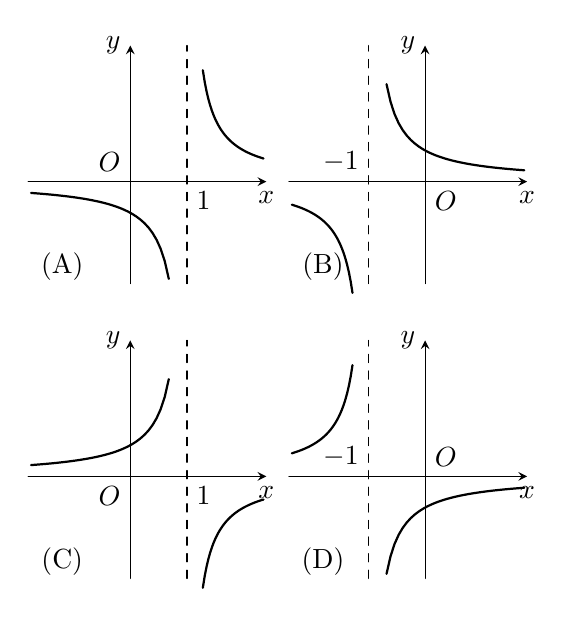
\begin{tikzpicture}[>=stealth,scale=0.72,line cap=round]
  % (A) 垂直渐近线 x = 1，双曲线递减分支
  \begin{scope}
    \draw[->] (-1.8,0)--(2.4,0) node[below] {$x$};
    \draw[->] (0,-1.8)--(0,2.4) node[left] {$y$};
    \node[above left] at (0,0) {$O$};
    \draw[dashed] (1,-1.8)--(1,2.4);
    \node[below right] at (1,0) {$1$};
    \draw[thick,domain=1.28:2.35,samples=35] plot (\x,{0.55/(\x-1)});
    \draw[thick,domain=-1.75:0.68,samples=35] plot (\x,{0.55/(\x-1)});
    \node at (-1.2,-1.5) {(A)};
  \end{scope}

  % (B) 垂直渐近线 x = -1，双曲线递减分支（正确选项）
  \begin{scope}[xshift=5.2cm]
    \draw[->] (-2.4,0)--(1.8,0) node[below] {$x$};
    \draw[->] (0,-1.8)--(0,2.4) node[left] {$y$};
    \node[below right] at (0,0) {$O$};
    \draw[dashed] (-1,-1.8)--(-1,2.4);
    \node[above left] at (-1,0) {$-1$};
    \draw[thick,domain=-0.68:1.75,samples=35] plot (\x,{0.55/(\x+1)});
    \draw[thick,domain=-2.35:-1.28,samples=35] plot (\x,{0.55/(\x+1)});
    \node at (-1.8,-1.5) {(B)};
  \end{scope}

  % (C) 垂直渐近线 x = 1，双曲线递增分支
  \begin{scope}[yshift=-5.2cm]
    \draw[->] (-1.8,0)--(2.4,0) node[below] {$x$};
    \draw[->] (0,-1.8)--(0,2.4) node[left] {$y$};
    \node[below left] at (0,0) {$O$};
    \draw[dashed] (1,-1.8)--(1,2.4);
    \node[below right] at (1,0) {$1$};
    \draw[thick,domain=1.28:2.35,samples=35] plot (\x,{-0.55/(\x-1)});
    \draw[thick,domain=-1.75:0.68,samples=35] plot (\x,{-0.55/(\x-1)});
    \node at (-1.2,-1.5) {(C)};
  \end{scope}

  % (D) 垂直渐近线 x = -1，双曲线递增分支
  \begin{scope}[xshift=5.2cm,yshift=-5.2cm]
    \draw[->] (-2.4,0)--(1.8,0) node[below] {$x$};
    \draw[->] (0,-1.8)--(0,2.4) node[left] {$y$};
    \node[above right] at (0,0) {$O$};
    \draw[dashed] (-1,-1.8)--(-1,2.4);
    \node[above left] at (-1,0) {$-1$};
    \draw[thick,domain=-0.68:1.75,samples=35] plot (\x,{-0.55/(\x+1)});
    \draw[thick,domain=-2.35:-1.28,samples=35] plot (\x,{-0.55/(\x+1)});
    \node at (-1.8,-1.5) {(D)};
  \end{scope}
\end{tikzpicture}\end{center}
\nopagebreak[4]
\end{question}
\begin{question}
\gkti{3}已知函数 $y = \sin\left(x - \dfrac{\pi}{12}\right)\cos\left(x - \dfrac{\pi}{12}\right)$，则下列判断正确的是\mbox{（　　）}

\begin{gkopts}(1)
\task A．此函数的最小正周期为 $2\pi$，其图象的一个对称中心是 $\left(\dfrac{\pi}{12}, 0\right)$
\task B．此函数的最小正周期为 $\pi$，其图象的一个对称中心是 $\left(\dfrac{\pi}{12}, 0\right)$
\task C．此函数的最小正周期为 $2\pi$，其图象的一个对称中心是 $\left(\dfrac{\pi}{6}, 0\right)$
\task D．此函数的最小正周期为 $\pi$，其图象的一个对称中心是 $\left(\dfrac{\pi}{6}, 0\right)$
\end{gkopts}

\end{question}
\begin{question}
\gkti{4}下列函数既是奇函数，又在区间 $[-1, 1]$ 上单调递减的是\mbox{（　　）}

\begin{gkopts}(2)
\task A．$f(x) = \sin x$
\task B．$f(x) = -|x + 1|$
\task C．$f(x) = \dfrac{1}{2}(a^x + a^{-x})$
\task D．$f(x) = \ln \dfrac{2-x}{2+x}$
\end{gkopts}

\end{question}
\begin{question}
\gkti{5}如果 $\left(3x - \dfrac{1}{\sqrt[3]{x^2}}\right)^n$ 的展开式中各项系数之和为 $128$，则展开式中 $\dfrac{1}{x^3}$ 的系数是\mbox{（　　）}

\begin{gkopts}(4)
\task A．$7$
\task B．$-7$
\task C．$21$
\task D．$-21$
\end{gkopts}

\end{question}
\begin{question}
\gkti{6}函数 $f(x) = \begin{cases} \sin(\pi x^2), & -1 < x < 0, \\ \mathrm{e}^{x-1}, & x \geqslant 0. \end{cases}$ 若 $f(1) + f(a) = 2$，则 $a$ 的所有可能值为\mbox{（　　）}

\begin{gkopts}(2)
\task A．$1$
\task B．$-\dfrac{\sqrt{2}}{2}$
\task C．$1, -\dfrac{\sqrt{2}}{2}$
\task D．$1, \dfrac{\sqrt{2}}{2}$
\end{gkopts}

\end{question}
\begin{question}
\gkti{7}已知向量 $\vec{a}, \vec{b}$，且 $\vec{AB} = \vec{a} + 2\vec{b}$，$\vec{BC} = -5\vec{a} + 6\vec{b}$，$\vec{CD} = 7\vec{a} - 2\vec{b}$，则一定共线的三点是\mbox{（　　）}

\begin{gkopts}(2)
\task A．$A$、$B$、$D$
\task B．$A$、$B$、$C$
\task C．$B$、$C$、$D$
\task D．$A$、$C$、$D$
\end{gkopts}

\end{question}
\begin{question}
\gkti{8}设地球的半径为 $R$，若甲地位于北纬 $45^\circ$ 东经 $120^\circ$，乙地位于南纬 $75^\circ$ 东经 $120^\circ$，则甲、乙两地的球面距离为\mbox{（　　）}

\begin{gkopts}(2)
\task A．$\sqrt{3}R$
\task B．$\dfrac{\pi}{6}R$
\task C．$\dfrac{5\pi}{6}R$
\task D．$\dfrac{2\pi}{3}R$
\end{gkopts}

\end{question}
\begin{question}
\gkti{9}$10$ 张奖券中只有 $3$ 张有奖，$5$ 个人购买，每人 $1$ 张，至少有 $1$ 人中奖的概率是\mbox{（　　）}

\begin{gkopts}(4)
\task A．$\dfrac{3}{10}$
\task B．$\dfrac{1}{12}$
\task C．$\dfrac{1}{2}$
\task D．$\dfrac{11}{12}$
\end{gkopts}

\end{question}
\begin{question}
\gkti{10}设集合 $A$、$B$ 是全集 $U$ 的两个子集，则 $A \subsetneqq B$ 是 $(\complement_U A) \cup B = U$ 的\mbox{（　　）}

\begin{gkopts}(2)
\task A．充分不必要条件
\task B．必要不充分条件
\task C．充要条件
\task D．既不充分也不必要条件
\end{gkopts}

\end{question}
\begin{question}
\gkti{11}$0 < a < 1$，下列不等式一定成立的是\mbox{（　　）}

\begin{gkopts}(1)
\task A．$|\log_{1+a} (1-a)| + |\log_{1-a} (1+a)| > 2$
\task B．$|\log_{1+a} (1-a)| < |\log_{1-a} (1+a)|$
\task C．$|\log_{1+a} (1-a) + \log_{1-a} (1+a)| < |\log_{1+a} (1-a)| + |\log_{1-a} (1+a)|$
\task D．$|\log_{1+a} (1-a) - \log_{1-a} (1+a)| < |\log_{1+a} (1-a)| - |\log_{1-a} (1+a)|$
\end{gkopts}

\end{question}
\begin{question}
\gkti{12}设直线 $l: 2x + y + 2 = 0$ 关于原点对称的直线为 $l'$，若 $l'$ 与椭圆 $x^2 + \dfrac{y^2}{4} = 1$ 的交点为 $A$、$B$，点 $P$ 为椭圆上的动点，则使 $\triangle PAB$ 的面积为 $\dfrac{1}{2}$ 的点 $P$ 的个数为\mbox{（　　）}

\begin{gkopts}(4)
\task A．$1$
\task B．$2$
\task C．$3$
\task D．$4$
\end{gkopts}

\end{question}
\gkpart{二、填空题：本大题共 4 小题，每小题 4 分，共 16 分．把答案填在题中横线上．}

\begin{question}
\gkti{13}$\lim_{n \to \infty} \dfrac{\mathrm{C}_n^2 + 2\mathrm{C}_n^{n-2}}{(n+1)^2} = \underline{\hspace{2em}}$．

\end{question}
\begin{question}
\gkti{14}设双曲线 $\dfrac{x^2}{a^2} - \dfrac{y^2}{b^2} = 1\ (a > 0, b > 0)$ 的右焦点为 $F$，右准线 $l$ 与两条渐近线交于 $P$、$Q$ 两点，如果 $\triangle PQF$ 是直角三角形，则双曲线的离心率 $e = \underline{\hspace{2em}}$．

\end{question}
\begin{question}
\gkti{15}设 $x, y$ 满足约束条件 $\begin{cases} x + y \leqslant 5, \\ 3x + 2y \leqslant 12, \\ 0 \leqslant x \leqslant 3, \\ 0 \leqslant y \leqslant 4, \end{cases}$ 则使得目标函数 $z = 6x + 5y$ 最大的点 $(x, y)$ 是 $\underline{\hspace{2em}}$．

\end{question}
\begin{question}
\gkti{16}已知 $m, n$ 是不同的直线，$\alpha, \beta$ 是不重合的平面，给出下列命题：
① 若 $\alpha \parallel \beta$，$m \subset \alpha$，$n \subset \beta$，则 $m \parallel n$；
② 若 $m, n \subset \alpha$，$m \parallel \beta$，$n \parallel \beta$，则 $\alpha \parallel \beta$；
③ 若 $m \perp \alpha$，$n \perp \beta$，$m \parallel n$，则 $\alpha \parallel \beta$；
④ $m, n$ 是两条异面直线，若 $m \parallel \alpha$，$m \parallel \beta$，$n \parallel \alpha$，$n \parallel \beta$，则 $\alpha \parallel \beta$．
上面的命题中，真命题的序号是 $\underline{\hspace{2em}}$．（写出所有真命题的序号）

\end{question}
\gkpart{三、解答题：本大题共 6 小题，共 74 分．解答应写出文字说明、证明过程或演算步骤．}

\begin{question}
\gkti{17}已知向量 $\vec{m} = (\cos\theta, \sin\theta)$ 和 $\vec{n} = (\sqrt{2}-\sin\theta, \cos\theta)$，$\theta \in (\pi, 2\pi)$，且 $|\vec{m} + \vec{n}| = \dfrac{8\sqrt{2}}{5}$，求 $\cos\left(\dfrac{\theta}{2} + \dfrac{\pi}{8}\right)$ 的值．

\end{question}
\begin{question}
\gkti{18}袋中装有黑球和白球共 $7$ 个，从中任取 $2$ 个球都是白球的概率为 $\dfrac{1}{7}$，现有甲、乙两人从袋中轮流摸取 $1$ 球，甲先取，乙后取，然后甲再取 $\cdots\cdots$，取后不放回，直到两人中有一人取到白球时既终止．每个球在每一次被取出的机会是等可能的，用 $\xi$ 表示取球终止所需要的取球次数．
(1) 求袋中所有的白球的个数；
(2) 求随机变量 $\xi$ 的概率分布；
(3) 求甲取到白球的概率．

\end{question}
\begin{question}
\gkti{19}已知 $x = 1$ 是函数 $f(x) = mx^3 - 3(m+1)x^2 + nx + 1$ 的一个极值点，其中 $m, n \in \mathbf{R}$，$m < 0$．
(1) 求 $m$ 与 $n$ 的关系式；
(2) 求 $f(x)$ 的单调区间；
(3) 当 $x \in [-1, 1]$ 时，函数 $y = f(x)$ 的图象上任意一点的切线斜率恒大于 $3m$，求 $m$ 的取值范围．

\Needspace{0.4\textheight}
\end{question}
\begin{question}
\gkti{20}如图，已知长方体 $ABCD - A_1B_1C_1D_1$，$AB = 2$，$AA_1 = 1$，直线 $BD$ 与平面 $AA_1B_1B$ 所成的角为 $30^\circ$，$AE$ 垂直 $BD$ 于 $E$，$F$ 为 $A_1B_1$ 的中点．
(1) 求异面直线 $AE$ 与 $BF$ 所成的角；
(2) 求平面 $BDF$ 与平面 $AA_1B$ 所成的二面角（锐角）的大小；
(3) 求点 $A$ 到平面 $BDF$ 的距离．
\nopagebreak[4]
\begin{center}% 2005 年山东卷理科第 20 题：长方体直观图与辅助线
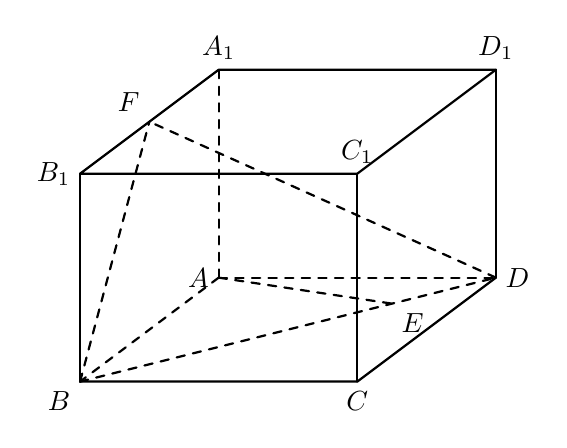
\begin{tikzpicture}[>=stealth,scale=1.1,line cap=round,line join=round]
  % 坐标定义
  % 底面顶点
  \coordinate (A) at (0,0);
  \coordinate (B) at (-1.6,-1.2);
  \coordinate (C) at (1.6,-1.2);
  \coordinate (D) at (3.2,0);

  % 顶面顶点（竖直高度 2.4）
  \coordinate (A1) at (0,2.4);
  \coordinate (B1) at (-1.6,1.2);
  \coordinate (C1) at (1.6,1.2);
  \coordinate (D1) at (3.2,2.4);

  % 中点与垂足
  \coordinate (F) at (-0.8,1.8); % A1B1 中点
  \coordinate (E) at (2.0,-0.3); % AE 垂直 BD 于 E (落在 CC1 右后方)

  % 虚线（不可见棱与辅助线）
  \draw[dashed,thick] (A) -- (A1);
  \draw[dashed,thick] (A) -- (B);
  \draw[dashed,thick] (A) -- (D);
  \draw[dashed,thick] (A) -- (E);
  \draw[dashed,thick] (B) -- (D);
  \draw[dashed,thick] (B) -- (F);
  \draw[dashed,thick] (D) -- (F);

  % 实线（可见棱）
  \draw[thick] (B) -- (C) -- (D);
  \draw[thick] (B) -- (B1);
  \draw[thick] (C) -- (C1);
  \draw[thick] (D) -- (D1);
  \draw[thick] (A1) -- (B1) -- (C1) -- (D1) -- cycle;

  % 顶点标签
  \node[above] at (A1) {$A_1$};
  \node[above] at (D1) {$D_1$};
  \node[left] at (B1) {$B_1$};
  \node[above] at (C1) {$C_1$};
  \node[above left] at (F) {$F$};
  \node[left] at (A) {$A$};
  \node[right] at (D) {$D$};
  \node[below left] at (B) {$B$};
  \node[below] at (C) {$C$};
  \node[below right] at (E) {$E$};
\end{tikzpicture}\end{center}
\nopagebreak[4]
\end{question}
\begin{question}
\gkti{21}已知数列 $\{a_n\}$ 的首项 $a_1 = 5$，前 $n$ 项和为 $S_n$，且 $S_{n+1} = 2S_n + n + 5\ (n \in \mathbf{N}^*)$．
(1) 证明数列 $\{a_n + 1\}$ 是等比数列；
(2) 令 $f(x) = a_1 x + a_2 x^2 + \cdots + a_n x^n$，求函数 $f(x)$ 在点 $x = 1$ 处的导数 $f'(1)$ 并比较 $2f'(1)$ 与 $23n^2 - 13n$ 的大小．

\end{question}
\begin{question}
\gkti{22}已知动圆过定点 $\left(\dfrac{p}{2}, 0\right)$，且与直线 $x = -\dfrac{p}{2}$ 相切，其中 $p > 0$．
(1) 求动圆圆心 $C$ 的轨迹的方程；
(2) 设 $A$、$B$ 是轨迹 $C$ 上异于原点 $O$ 的两个不同点，直线 $OA$ 和 $OB$ 的倾斜角分别为 $\alpha$ 和 $\beta$，当 $\alpha, \beta$ 变化且 $\alpha + \beta$ 为定值 $\theta\ (0 < \theta < \pi)$ 时，证明直线 $AB$ 恒过定点，并求出该定点的坐标．

\end{question}